%!TEX root = ../../Physics_XES_II.tex
\chapterauthor{\sf 认识与描述物质的世界...}{}
%\chapterauthor{Second Author}{Second Author Affiliation}
\chapter{运动学}\label{2}

\emph{插图}

 

\section{时空与物质}\label{2-1}

物理学, 从刚开始成为实验性的科学的伽利略时期开始, 到近半个世纪年来理论物理学家对额外维度的探讨, 都给予了\emph{时空}(spacetime)最核心的地位. 牛顿的理论, 分析力学, 经典场论, 相对论这些理论最基本的图像都是时空与\emph{物质}(matter)的分立性. 时空是装备了一个能体现出物理物理意义的\emph{度量}(metric)的3+1维对象. 数学上有一套严格的说法, 把这种连续, 光滑的四维对象称为\emph{伪黎曼流形}(pseudo-Riemannian manifold). 而物质则是在每个时空点处的某种结构. 经典理论下, 这种结构不外乎用\emph{标量}(scalar), \emph{矢量}(vector)或是更高级的\emph{张量}(tensor)来描述. 最后, 这些量的变化就体现出了形形色色的\emph{运动}(motion). \emph{运动学}(kinematics)的主要任务就是描写物质的运动, 而对于物质运动背后体现出来的\emph{定律}(law), 我们仅做笼统的较浅的讨论, 更加深入地看, 不同物质运动符合的不同定律往往又需要因为时空的结构或相互作用的内禀属性而具有普遍的\emph{对称性}(symmetry), 对称性是``规律之规律'', 它对物理理论在何种程度上起到决定作用将是超出本书范围的更高层次的课题, 将伴随读者对物理学学习的生涯.

\subsection{时空观}\label{2-1-1}

牛顿力学理论体系基于\emph{伽利略时空观}(Galilean spacetime picture), 也就是\emph{绝对时空观}(absolute spacetime picture). 在这里空间是三维的平直空间. 设想一个人站在该空间的某个空间点, 他的胸前, 头顶和右手平举的三个方向就是相互垂直的方向. 如果以自己的臂长为标准长度, 他能够定义空间中每两个点之间的空间间隔. 事实上, 这个人能够以一种正确的方式为每个空间点定义一个坐标, 那么所有三维空间点的集合与任意两个点之间的距离为:

\[A(x,\,y,\,z)\in\mathbb{R}^3 \quad;\quad x,\,y,\,z\in\mathbb{R}\]
\[A(x_1,\,y_1,\,z_1)\;,\;B(x_2,\,y_2,\,z_2)\;:\;l^2=\overline{AB}^2=(x_1-x_2)^2+(y_1-y_2)^2+(z_1-z_2)^2\]

因为空间不同于时间, 我们为以上数字赋予特殊的物理含义, 也就是加上\emph{量纲}(dimension). 如果两点坐标为$(0,\,0,\,0)$和$(1,\,1,\,1)$, 那么$l=\sqrt{3}{\rm m}$, 而不是$l=\sqrt{3}$. 其单位${\rm m}$一方面表示了这个物理量的属性, 另一方面指定了某个实际物理体系确定下来的固有长度大小. 现行的(2018年1月1日, 下文同)国际单位制对$1{\rm m}$的定义如下\footnote{一方面, 它依赖于狭义相对论的正确性, 目前极少理论物理工作者会质疑它. 另一方面, 应该要先定义下文的1s, 再来定义1m.}:
\begin{verse}
1m是光在1/299792458 s内在真空中行进的距离.
\end{verse}


这就是我们的\emph{三维平直空间}(3-dimensional flat space). 注意空间点具有物理实际意义, 它可以脱离坐标系而单独存在. 事实上坐标系的原点可以建立在空间中的任意点处, 朝向也可以是任意方向, 两个空间点之间的距离$l$不会依赖于坐标系的选取, 但两个点的坐标会因坐标系不同而改变. 如果我们选取的坐标系总是下述使得两个相距很近的点之间的微元距离公式成立:
\[\ud l^2=\ud x^2+\ud y^2+\ud z^2\]


那么建立的坐标系就是一个\emph{笛卡尔坐标系}(Cartesian coordinate system), 即\emph{空间直角坐标系}(3D orthogonal coordinate system). 但是以空间直角坐标系为基础, 我们又经常建立\emph{球坐标}(spherical coordinate)和\emph{柱坐标}(cylindrical coordinate)系统. 通常取$x$轴为\emph{幅轴}(azimuth axis), 点在$x-y$平面上的投影与原点的连线相对$x$轴转过的角度为$\varphi$, 即\emph{幅角}(azimuth angle). 而$z$轴为\emph{极轴}(polar axis), 而点与原点连线与极轴的夹角$\theta$为\emph{极角}(polar angle). 天文观测用球坐标就很方便, 它是以描述的空间点到原点之间的距离$r$, 也称\emph{矢径}(radius), 和两个描述角位置的极角幅角来构成三个坐标$(r,\theta,\varphi)$的. 而理论物理里也常用到的柱坐标是以$(\rho,\varphi,z)$为描述空间点的坐标, $\rho$是空间点到$z$轴的距离.

\begin{wrapfigure}[20]{o}[-10pt]{7cm}
\vspace{-0.4cm}
\centering
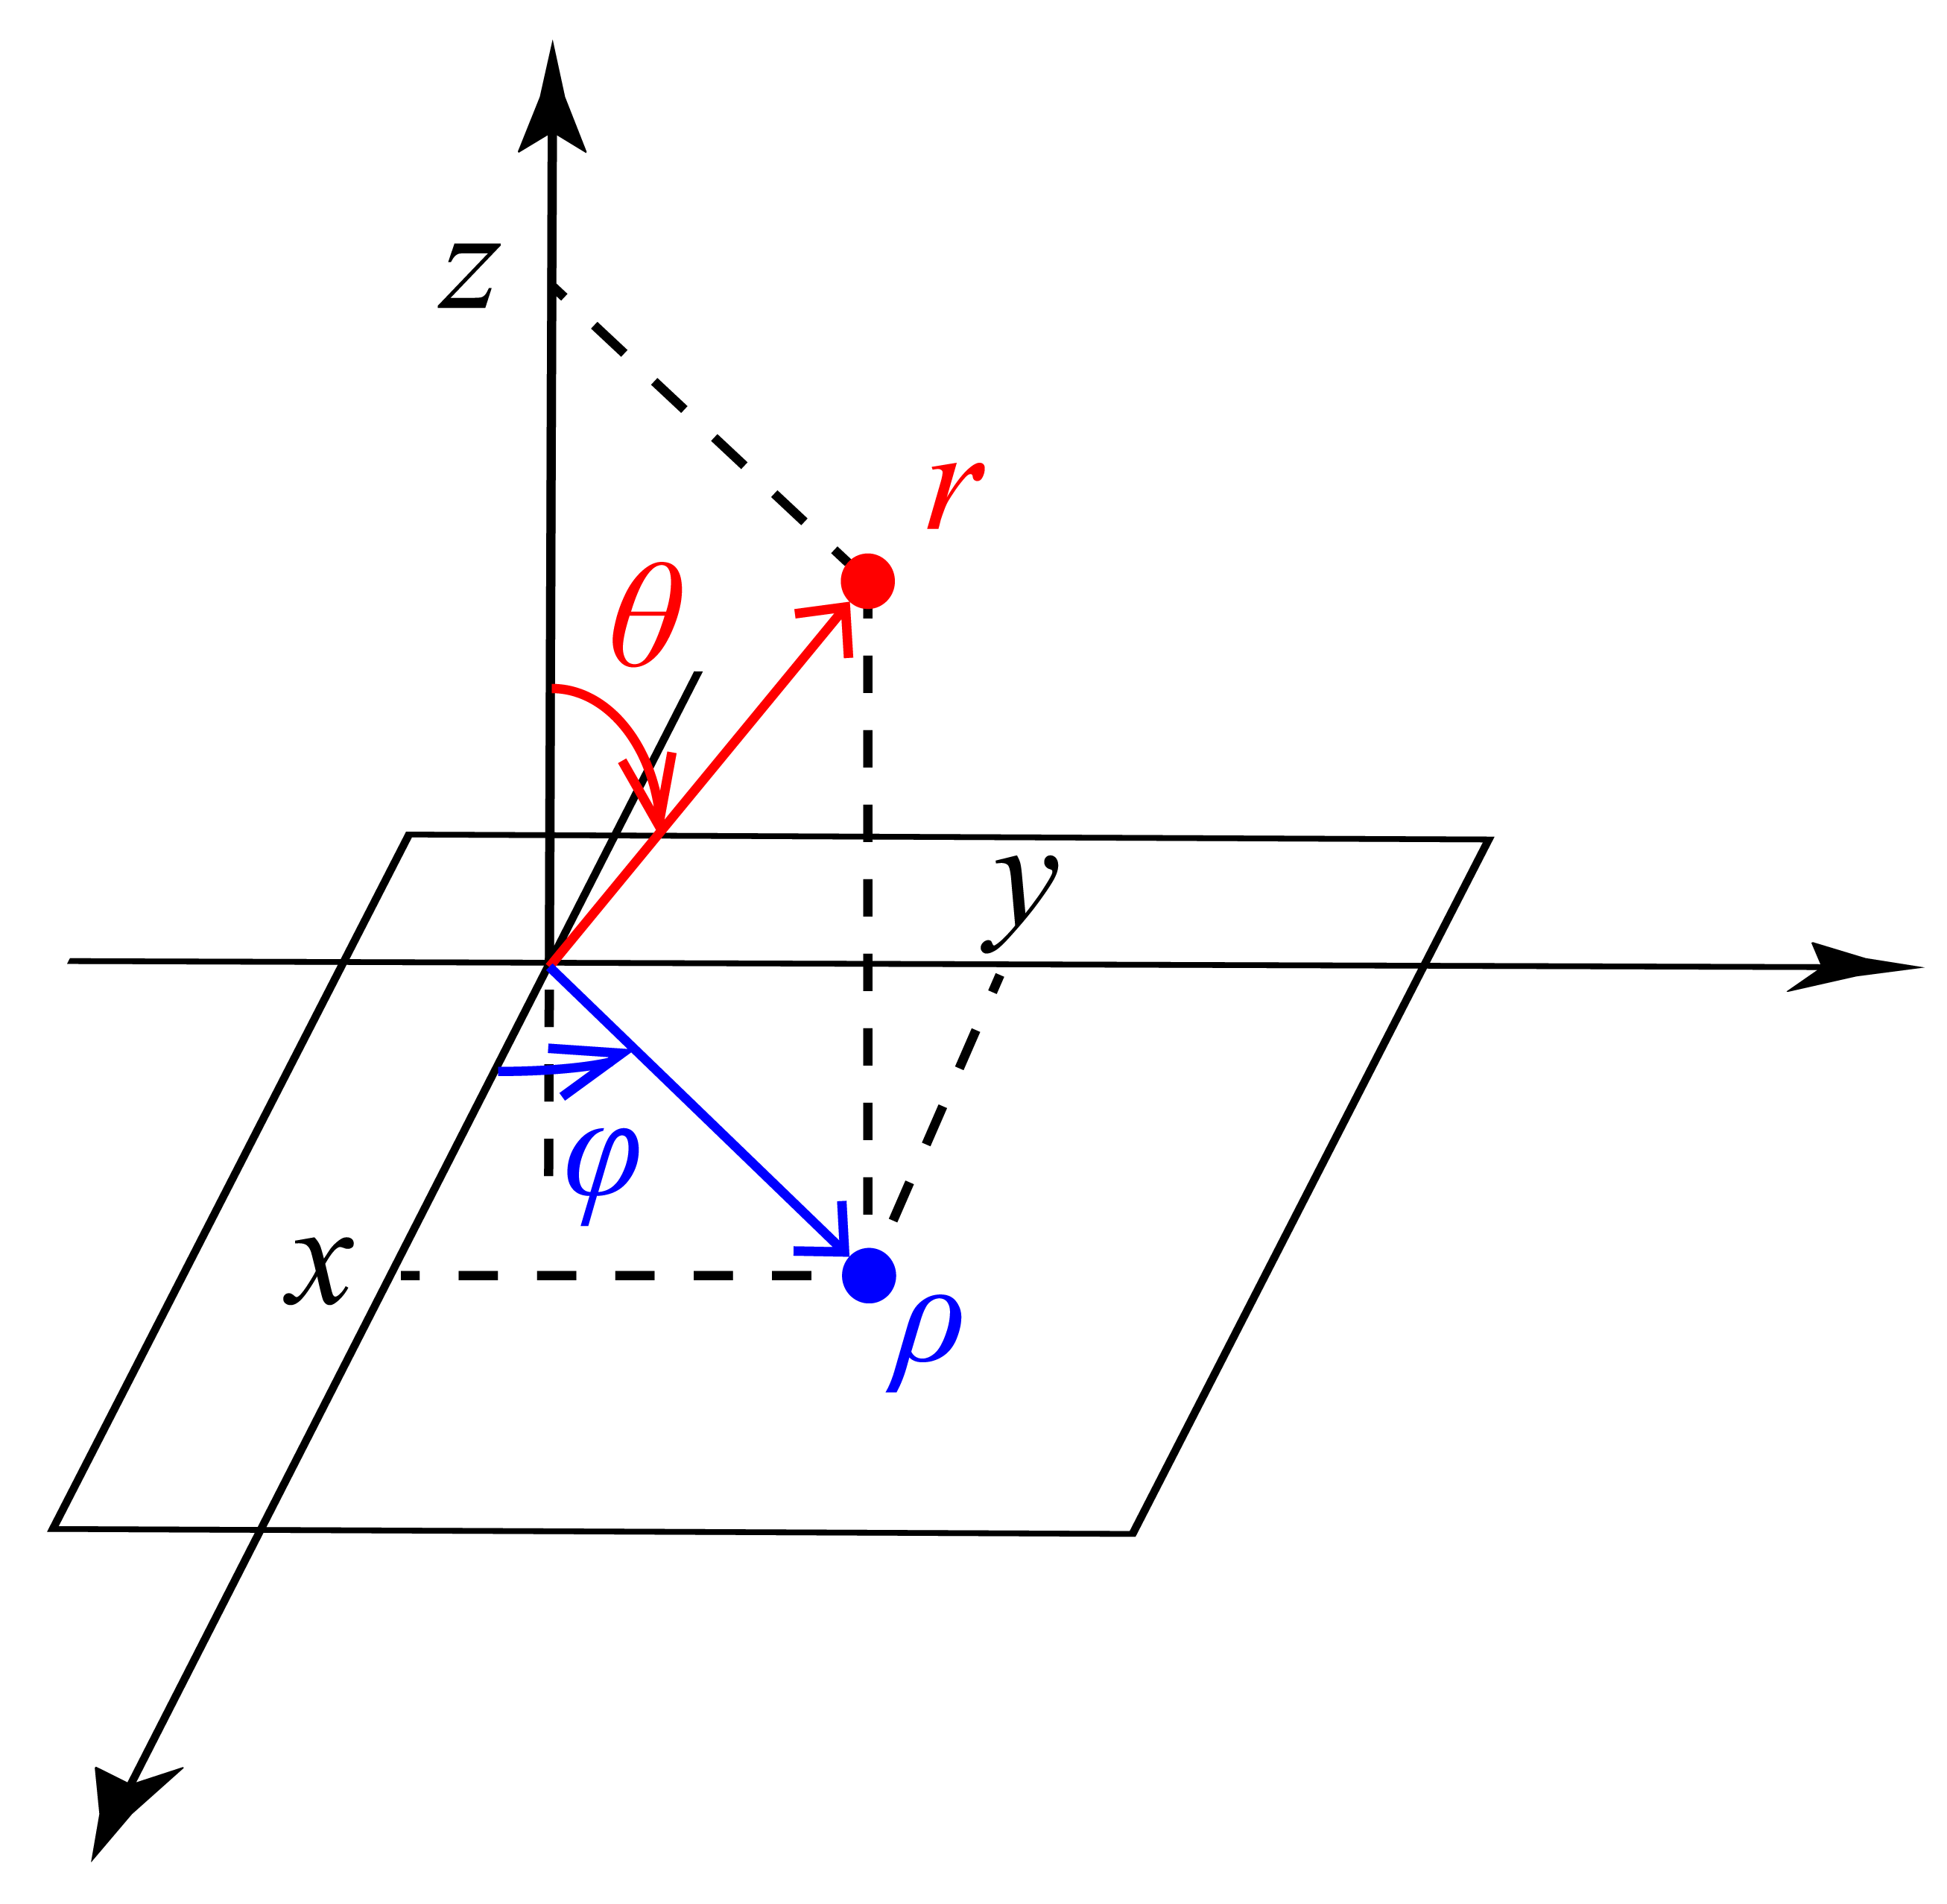
\includegraphics[width=7cm]{image/6-1-1.png}
\caption{三种坐标}
\end{wrapfigure}
需要注意, 我们对以上$\theta, \varphi$角度定义比较微妙, $\theta$一般限制其在$[0,\,\pi]$范围内, 在端点$\theta=0, \pi$处$\varphi$的不同取值代表同一个空间点. 但$\varphi$的取值我们不加以任何限制, 也就是原则上$\varphi\in\mathbb{R}$. 而任意$\varphi$相差$2n\pi$的坐标实际上代表同一个空间点. 这么做是因为我们最好不要用静态的几何观点去看待角度这一概念. 而是用运动, 变换的观点去看待角度. 作为连续的运动的点的幅角变化也应是连续的, 为了使点绕$z$轴一圈后幅角不至于突然改变, 就必须默认每一点的幅角可以有多种取值, 在具体的运动中应该灵活选择其具体取值大小.

之后经常会说到各种对称性, 在本系列教材中我们采取如下说法: \emph{球对称}(spherical symmetric)仅仅代表某个函数$f(r,\theta,\varphi)$与$\varphi$无关. 而\emph{柱对称}(cylindrical symmetric)代表的是$f(\rho,\varphi,z)$与$z$无关. 与$\varphi$和$\theta$都无关的$f(r,\theta,\varphi)=f(r,\forall\theta,\forall\varphi)$被称为\emph{各向同性}(isotropic). 最后\emph{中心对称}(centrosymmetric)是一个很弱的对称性, 它仅仅代表函数在\emph{中心反演}(space inversion)下的对称性:
\[f(x,y,z)=f(-x,-y,-z)\]

绝对时空观中的时间则是一种完全与空间独立的属性. 实际上, 每一个空间点处的人都能感受到时间的流逝. 十分抽象的把这些不同的时刻画在一根时间轴上, 便是一维的时间坐标:
\[A(t)\in\mathbb{R} \quad;\quad t\in\mathbb{R}\]

而时空又是两个独立的概念. 任意一个坐标点处都有时间轴, 而任意一个时刻都有一个三维空间切片. 事实上, 我们的时空是一个3+1维的结构, 合理地选取坐标后, 实际上可以把时空结构写成四维坐标:
\[A(x,\,y,\,z,\,t)\in\mathbb{R}^4 \quad;\quad x,\,y,\,z,\,t\in\mathbb{R}\]

而对于任意两个时空点, 存在绝对的时间, 也就是可以找到两个事件的绝对时间差:
\[\tau=|t_2-t_1|\]

但空间距离却具有相对性. 我们要求在同一时刻的同一空间切片上定义空间的度量:
\[t_1=t_2:\quad l=\sqrt{(x_1-x_2)^2+(y_1-y_2)^2+(z_1-z_2)^2}\]

不同时刻的空间, 被线性地组织在一起, 保证每一刻都平直的空间既不会随时间膨胀收缩, 也不会旋转加速. 这种时空结构被叫做\emph{牛顿-嘉当几何}(Newton-Cartan geometry)%\footnote{用更为严格的语言来说, 我们需要一个装备了一阶形式``钟''$c_\nu$和二阶逆变半正定对称张量类空间度规$s^{\mu\nu}$的四维微分流形$\mathscr{M}$:
%\[\mathscr{M}:\quad s^{\mu\nu}c_{\nu}=0\]}.

时间是一个新的量纲, 其国际单位制对$1{\rm s}$的定义为:
\begin{verse}
1s是铯-133原子基态的两个超精细能级之间跃迁所对应的辐射周期时长的9192631770倍.
\end{verse}

牛顿-嘉当几何的显著特点是物理量的定义没有所谓的\emph{协变性}(covariance). 固然, 在三维空间坐标框架的旋转下, 任何物理过程中的事件所发生的位置坐标发生旋转变换, 而几乎所有标量(比如质量, 能量)都不变, 几乎所有矢量(比如动量, 角动量)都按照类似坐标变换的法则发生变换. 但是, 对于更普遍的一列\emph{伽利略变换}(Galilean transformation), 也就是相对匀速运动的参考系之间的变换, 时空坐标的形式却不能简单地推广到能量动量角动量上.

不同于绝对时空观中时间与空间成为相互独立的量纲的特点, 狭义相对论改变了对基本物理量的看法. 狭义相对论把时空看成为可以相互转化的不可分割的新的3+1维整体, 同时性已然破缺. 两个时空点之间无法定义绝对的时间间隔. 在\emph{相对论时空观}(relativistic spacetime picture)下, 时间和空间可以用同一把尺子去丈量: 这是由于光速的不变性:
\[c=299792458{\rm m/s}\]

而量出来的长度叫做\emph{时空间隔}(spacetime interval):
\[\ud s^2=c^2\ud t^2-\ud x^2-\ud y^2-\ud z^2\]

这赋予时空以截然不同的结构, 最关键的一点是, 时间的绝对性被取消了, 不同事件发生时间先后的比较不总是可行, 相对论的有限速度因果律在这里取代了经典观点的时序因果律. 我们将在 电磁学理论的最后介绍相对论理论.

\subsection{物质观}\label{2-1-2}

\subsection{世界观}\label{2-1-3}